\documentclass[10pt,a4paper]{article}
\usepackage[utf8]{inputenc}
\bibliographystyle{unsrt}
\usepackage[pdftex]{graphicx}
\usepackage{hyperref}
% next one for links to point to the figure/table,
% not its caption
\usepackage[hypcap]{caption}

\begin{document}
\author{Pavlo Shchelokovskyy}
\title{Instability of bell shape in vesicles sedimenting under gravity}
\date{\today}
\maketitle

\abstract{The bell like shape for vesicles sedimenting under the gravity predicted previousely was observed.
The shape is in the agreement with the model given experimental parameters.
However it was found to be unstable contrary to theoretical predictions.
This instability may be attributed to thermal undulations of lipid membrane.}

\section{Introduction}\label{intro}
The sedimentation of giant lipid vesicles under gravity was studied in \cite{Huang2011}, observing pear-like shapes of tensionless deflated vesicles settling under gravity in the presence of density difference between inner media of the vesicle and outer solution.
Other shapes described include formation of tethers and pearl chains under these conditions.
Theoretical investigation of this system was carried out in \cite{Boedec2012}, where authors provided analytical and numerical solutions of the problem at hand, reproducing the spectrum of shape morphologies of the system.
Additionally, it was found that depending on the initial conditions sedimenting vesicle can attain a characteristic bell-like shape, not observed in the experiments before.

Here we report observation of such bell-like shaped sedimenting vesicles in our experiments, and further more compare the experimental results with theoretical predictions made in \cite{Boedec2012}.

\section{Materials and methods}\label{methods}

\subsection{Vesicle preparation and observation}
Vesicles were prepared from 1,2-dioleoyl-sn-glycero-3-phosphocholine \newline (DOPC) by electroformation method \cite{Angelova1986}.
Shortly, 5~$\mu$m of 4~mM solution of DOPC in chloroform (both \emph{Sigma-Aldrich Chemie GmbH, Steinheim, Germany}) were deposited on each of two ITO-covered glass slides (\emph{Sigma-Aldrich Co, St.Lois, USA}) and dried in desiccator at room temperature for 1 hour to evaporate the solvent.
Afterwards they were assembled in the chamber using 2~mm thick Teflon spacer.
The chamber was filled with 300~mM sucrose solution (\emph{Sigma-Aldrich Chemie GmbH, Steinheim, Germany}), sealed with silicone grease and subjected to AC field of 10~Hz at 3.1~V peak-to peak amplitude for the duration of 1 hour with the help of TGA1230 function generator (\emph{Thurlby Thandar Instruments, Huntingdon, UK}).
The procedure was finished with applying the AC field of 5~Hz and peak-to-peak amplitude of 3.6~V for another 20 minutes to detach vesicles from the glass.

Vesicles solution was then collected and diluted with solution of either 335~mM glucose (\emph{Sigma-Aldrich Chemie GmbH, Steinheim, Germany}) and 0.01~mM NaCl (\emph{Fluka Chemie AG, Buchs, Switzerland}) or 315~mM glucose and 0.094~mM NaCl in the volume proportion of vesicle solution to glucose-NaCl solution as 1:10 to provide for density, osmolarity, conductivity and optical density contrast.
The values of density and viscosity for those two solutions were found not to significantly differ from one another, and in the further analysis we use values of 1020.5~mg/ml for density and 1.1 mPa~s for the viscosity of the outer medium.
The density of the inner medium was measured to be 1039 mg/ml, making the density gradient to be 18.5~mg/ml. Viscosity was measured using Haake MARS~III rheometer (\emph{Thermo Fisher Scientific Inc, Waltham, MA, USA}).
This mix was then left for 15~minutes to sediment in the tube, separating bigger vesicles from the rest.
The final sample was collected form the bottom of the tube, and filled in the experimental chamber.
After that the unsealed chamber was left to evaporate in the room conditions for another 5 minutes in order to slowly change the osmolarity contrast and thus gently deflate vesicles.
Then the chamber was sealed.
Deionized water provided by Millipore Simplicity system (\emph{EMD Millipore, Billerica, USA}) was used in all solutions.

Vesicles were observed using tilted Olympus IX-70 microscope with Olympus LCPlanFI 40x objective and eco285M~VGE camera \newline (\emph{SVS-VISTEK GmbH, Seefeld, Germany}) with final image resolution of 0.135~$mu$m per pixel in phase contrast mode.
Experiments were carried out using in-house developed LabVIEW software for image acquisition. Images were saved with exposure time of 100~ms at frame rate of 9.9 per second.

\subsection{Electrodeformation of sedimenting vesicles}

In order to obtain initial condition for sedimenting vesicles as oblate ellipsoid we used method of electrodeformation in the AC field utilizing effect described in \cite{Aranda2008}.
We used custom made Teflon chambers with cavity of 10x5x2~mm and two parallel 0.8~mm thick copper electrodes positioned with approximately 7~mm distance between them and close to the glass (see Figure~\ref{fig:chamber}).
The AC field was supplied through the TGA1230 generator and WM-300 high voltage amplifier (\emph{Falco Systems, Amsterdam, Netherlands}), the former being driven by in-house developed software.
Electrodeformation was achieved by applying the AC field of approx. 130~V$_\mathrm{RMS}$ amplitude and frequency of 100~kHz in pulses of 100~ms (to decrease magnetohydrodynamic effects).

\begin{figure}
 \centering
 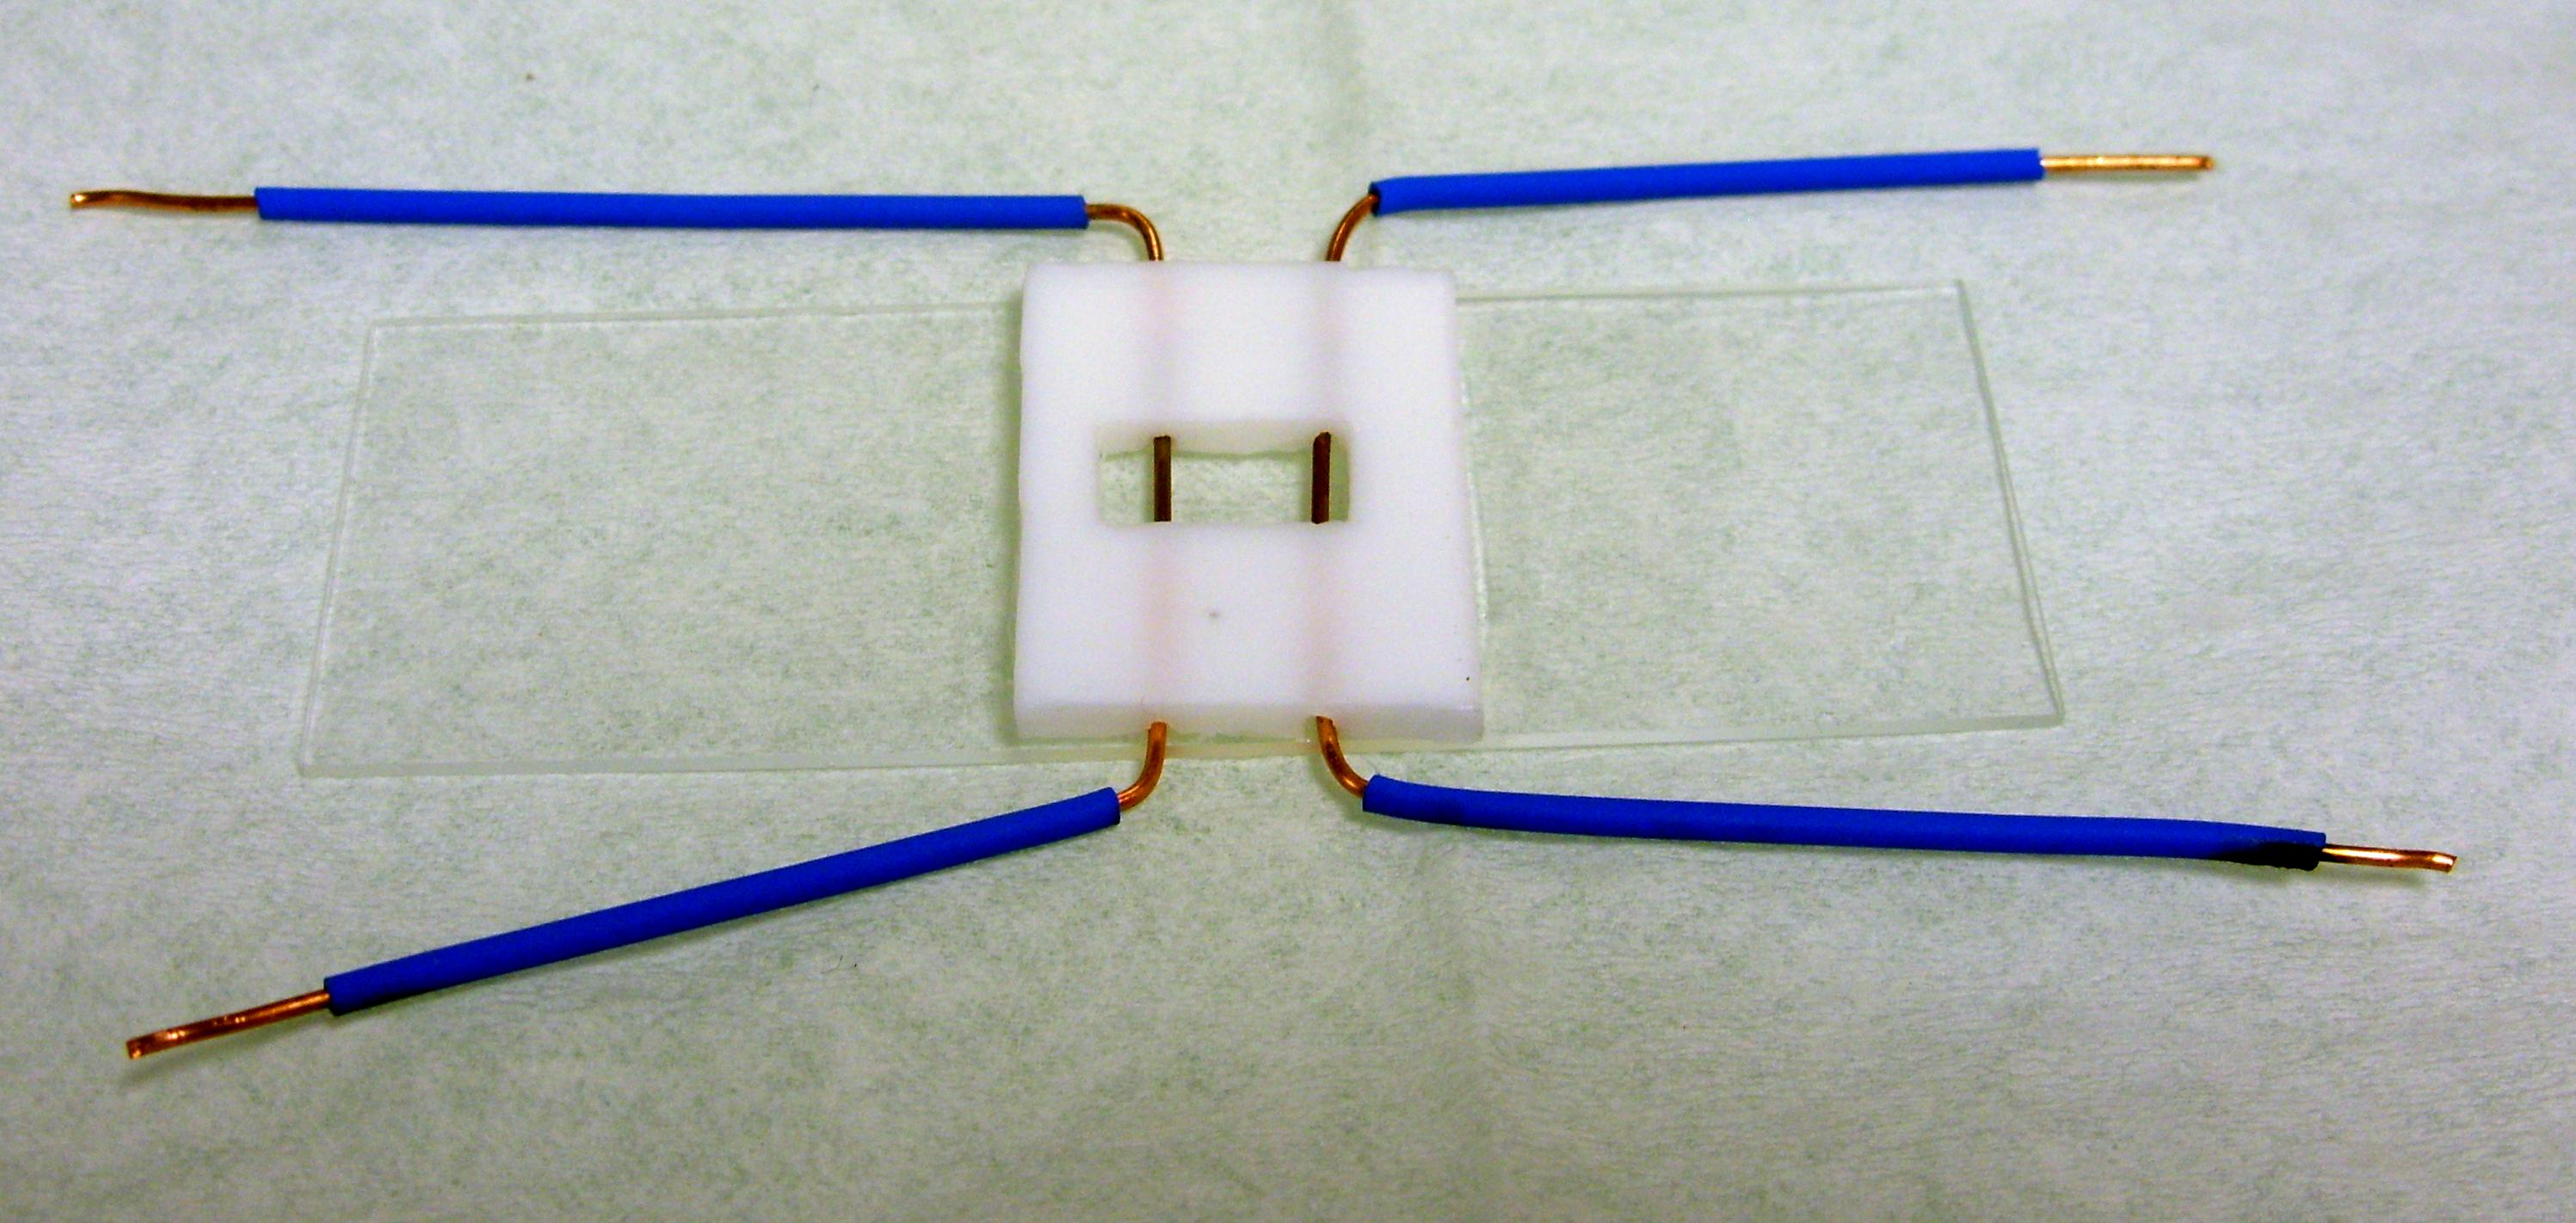
\includegraphics[width=0.7\linewidth]{figs/electro-chamber}
 \caption{Photo of the electrodeformation chamber.}\label{fig:chamber}
\end{figure}

\subsection{Image analysis}
The recorded images were analysed to extract the contour of the vesicle using ImageJ software \cite{ImageJ}.
Then we extracted the volume $V$, surface area $A$, the radius of equivolumetric sphere $R_0 = \sqrt[3]{\frac{3V}{4\pi}}$ and the excess area parameter $\Delta = \frac{A}{R_0^2} - 4\pi$ from the contour considering half of it as a solid of rotation.
As the vesicle was usually fluctuating and not exhibiting exactly symmetric shape, each of the halves in respect to approximate axis of symmetry was analysed separately, and final values for $V$ and $A$ were taken as an average between bodies of rotation corresponding to those two halves.

\section{Results}\label{results}
By using pulses of AC field as described and the geometry of our chamber we were able to obtain the initial shape of sedimenting vesicle as oblate ellipsoid, with axis parallel to the gravity direction.
Such vesicles do indeed initially exhibit the bell-like shape when sedimenting as predicted in \cite{Boedec2012}.

% !TeX root = bellshape.tex
\begin{table}
\centering
\begin{tabular}{|c|c|c|c|}
\hline
image & $V$, px$^3$ & $R_0$, px & $\Delta$\\ 
\hline
1 & 6785408.16276409 & 117.44353707894 & 0.945358727345529\\ 
\hline
2 & 3054119.19494 & 90.0048248442 & 1.16677966944\\ 
\hline
3 & 3464404.38872 & 93.8670833447 & 1.17766513303\\ 
\hline
4 & 5698269.44977 & 110.80298426 & 0.864513407125\\ 
\hline
5 & 4853469.528877 & 105.031902626382 & 1.00641564566709\\ 
\hline
6 & 3160856.37614 & 91.0413560364 & 1.00748951728\\ 
\hline
7 & 2574899.60436 & 85.0270732676 & 0.733848912512\\ 
\hline
8 & 2656007.1491 & 85.910624654 & 1.0058570969\\ 
\hline
9 & 6152539.55869 & 113.672462555 & 0.768597935549\\ 
\hline
10 & 4329241.38755 & 101.105410648 & 0.871477231082\\ 
\hline
11 & 2969904.61507 & 89.1698351957 & 1.10364565739\\ 
\hline
12 & 1678848.78812 & 73.7294494115 & 1.41350320422\\ 
\hline\end{tabular}
\caption{\small{Experimental data. Viscosity of the outer medium $\mu$ is 1.1 mPa~s. Density contrast $\Delta\rho$ is 18.5 mg/ml.}}
\label{tab:experiment} 
\end{table}

\subsection{Comparison with theoretical predictions}
Using values of $\Delta\rho$, $V$ and $\Delta$ from our experiments as input parameters (see Table \ref{tab:experiment}), we carried out the simulation procedure from \cite{Boedec2012}.

One also needs to consider an effect of sugars on bending rigidity, which enters the definition of Bond number.
At small sugar concentrations the bending rigidity $\kappa$ of the DOPC bilayer is known to be around $8\times10^{-20}$~J.
But as was shown in \cite{Vitkova2006} for SOPC and observed in \cite{Shchelokovskyy2011} for DOPC, the presence of sugars can drastically decrease the bending rigidity of the bilayer. 
Extrapolation data for SOPC from \cite{Vitkova2006} to our system with DOPC suggests that a more accurate value for the bending rigidity in the of presence of 300 mM sucrose solution is about 5~$k_\mathrm{B}T$, i.e $2\times10^{-20}$~J.

\subsection{Instability}
But it turns out that this morphology is not stable. After some time most vesicles morphed to pear-like shape (frequently followed by pearling).

\section{Discussion}\label{discussion}
The course of this change strongly suggests that thermal undulations of the membrane, which were not considered in the modeling of \cite{Boedec2012}, in fact play a crucial role, destabilizing the bell-like shape and making it a meta-stable morphology. Further refinement of the numerical model is needed to get insights into this transition.

\bibliography{bellshape}
\end{document}